\documentclass[a4paper,12pt]{article} 


\usepackage[T2A]{fontenc}			
\usepackage[utf8]{inputenc}			
\usepackage[english,russian]{babel}	

\usepackage{graphicx, scalerel}    
\usepackage{wrapfig}               
\usepackage[14pt]{extsizes}        
\usepackage[warn]{mathtext}       
\usepackage{indentfirst}      
\usepackage[margin = 25mm]{geometry}
\usepackage[table,xcdraw]{xcolor} 
\usepackage{amsmath,amsfonts,amssymb,amsthm,mathtools}
\usepackage{wasysym}                
\usepackage{upgreek}                
\usepackage{caption}
\usepackage{multirow}
\captionsetup{labelsep=period}
\usepackage[font=small,labelfont=bf]{caption}
\usepackage{gensymb}
\usepackage[unicode, pdftex]{hyperref}
\usepackage{tikz}
\usetikzlibrary{positioning}
\usepackage{fancyhdr}
\pagestyle{fancy}
\setlength\fboxsep{3pt} % Отступ рамки \fbox{} от рисунка
\setlength\fboxrule{1pt} % Толщина линий рамки \fbox{}
\newcommand{\tocsection}[1]{\section*{#1} \addcontentsline{toc}{section}{#1}}
\newcommand{\tocsubsection}[1]{\subsection*{#1} \addcontentsline{toc}{subsection}{#1}}
\renewcommand{\cftsecleader}{\cftdotfill{\cftdotsep}}

\begin{document}
		\newcommand{\HRule}{\rule{\linewidth}{0.7mm}} % Defines a new command for the horizontal lines, change thickness here

\begin{center}
	\large\textbf{Московский Физико-Технический Институт}\\
	\large\textbf{(государственный университет)}
	
	\vfill
	

	
	\Large Вычислительная математика
	%----------------------------------------------------------------------------------------
	%	TITLE SECTION
	%----------------------------------------------------------------------------------------
	
	\HRule
	\\[0.4cm]
	{ \huge \bfseries Лабораторная работа №9}
	\\[0.4cm] % Title of your document
	\HRule
	\\[0.5cm]
	
	\ \\
	\textbf{\large Автор:} \\	
	\large Овсянников Михаил Б01-008\\
	\vfill
	\hspace*{-0.8 cm}
\includegraphics[width=100 pt]{./Include/frkt_logo.pdf}\\
	\large Долгопрудный, 2023
\end{center}

\thispagestyle{empty}

\newpage
\setcounter{page}{2}
\fancyfoot[c]{\thepage}
\fancyhead[L] {Лабораторная работа №9}
\fancyhead[R]{}

		\tableofcontents
		\newpage
		
		\tocsection{Цель}
		Проанализировать и реализовать различные методы численного интегрирования функции. В частности, функции, заданной табличным способом. 

		\tocsection{Теоретические сведения}
		\tocsubsection{Общая задача}
		Задача численного интегрирования является очень острой и имеет огромное количество применений. Именно поэтому развита целая теория численного интегрирования, и существует множество формул, по которым можно посчитать интеграл заданной функции. 
		
		Общая задача ставится следующим образом. Пусть у нас есть некая функция $f(x)$, которая задана на каком-то промежутке $[x_0, x_n]$. Требуется найти следующий интеграл:
		\begin{equation*}
			I = \int\limits_{x_0}^{x_n} f(x) dx
		\end{equation*}
		Самое банальное, что сразу же приходит на ум, -- это разбить интервал интегрирования на элементарные отрезки $[x_k, x_{k+1}]$, $k = \overline{0, n-1}$ и представить функцию на каждом частичном отрезке как
		\begin{equation}
			f(x) = P_m (x) + R_m (x),
			\label{Poly}
		\end{equation}
		\noindent где $P_m (x)$ -- это многочлен степени не выше $m$, а $R_m$ -- это член ошибки.
		Перебирая различные $m$, мы сможем получать разные формулы численного интегрирования.
		
		\newpage
		\tocsubsection{Метод прямоугольников}
		Если в формуле \eqref{Poly} мы будем использовать $m = 0$, то получим так называемый метод прямоугольников.
		
		\begin{figure}[h!]
			\begin{minipage}[h]{0.49\linewidth}
				\center{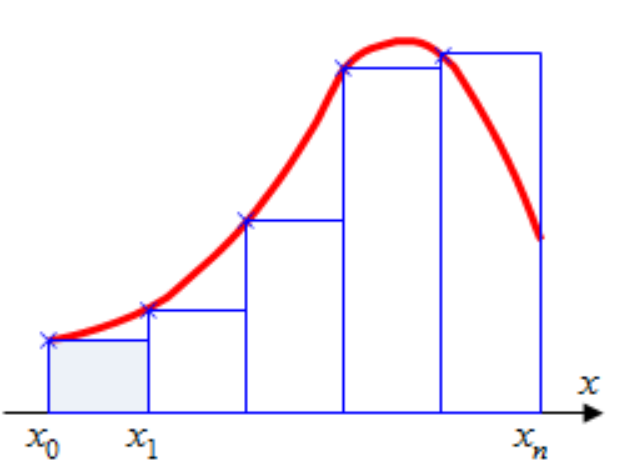
\includegraphics[width=0.9\linewidth]{Pictures/LeftRect} \\ а)}
			\end{minipage}
			\hfill
			\begin{minipage}[h]{0.49\linewidth}
				\center{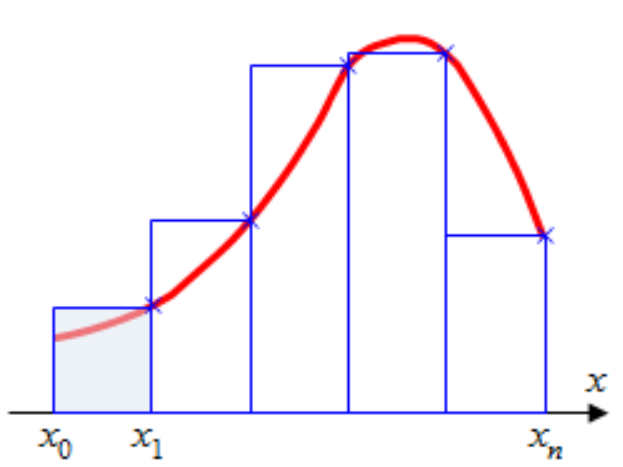
\includegraphics[width=0.9\linewidth]{Pictures/RightRect} \\ б)}
			\end{minipage}
			\caption{Метод прямоугольников: a) левых; б) правых}
			\label{Rects}
		\end{figure}
	
		Таким образом, мы приближаем нашу функцию константой на каждом элементарном интервале. Данный метод имеет первый порядок. Существуют две разновидности метода прямоугольников первого порядка -- левые и правые прямоугольники (Рис. \ref{Rects}). При равномерной сетке с шагом $h$ формулы
		\begin{equation}
			I = \int\limits_{x_0}^{x_n} f(x) dx \approx h\sum\limits_{k = 0}^{n-1}f_k
		\end{equation}
		\begin{equation}
			I = \int\limits_{x_0}^{x_n} f(x) dx \approx h\sum_{k = 1}^n f_k
		\end{equation}
		для левых и правых прямоугольников соответственно.
		
		Ошибка при подсчете методом прямоугольников дается формулой:
		\begin{equation}
			|R(f)| \leqslant \max\limits_{[x_0, x_n]}|f'(x)| \cdot \frac{x_n - x_0}{2}h
		\end{equation}
	
		
		\newpage
		\tocsubsection{Метод трапеций}
		Теперь берем $m = 1$ и получаем метод трапеций. Мы приближаем нашу функцию прямой на каждом элементарном отрезке (Рис. \ref{Trapez}).
		\begin{figure}[h!]
			\centering
			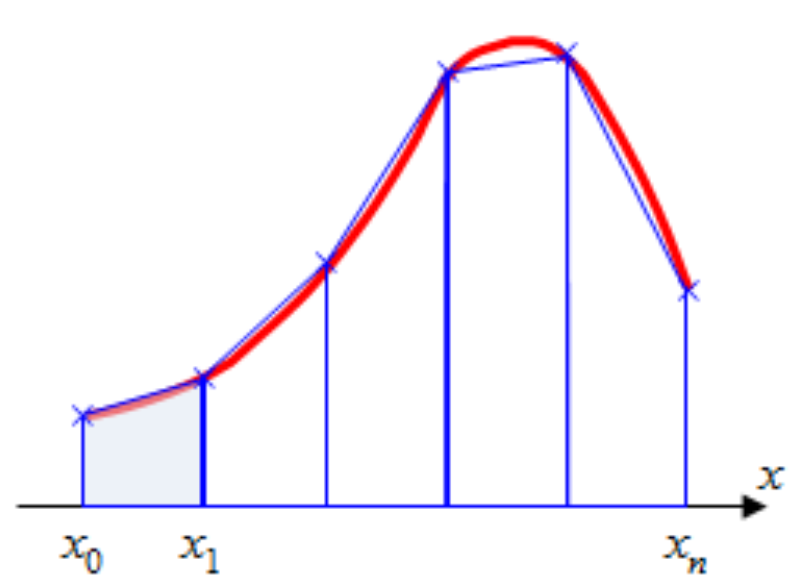
\includegraphics[width=0.65\linewidth]{Pictures/Trapez}
			\caption{Метод трапеций}
			\label{Trapez}
		\end{figure}
		
		Порядок этого метода -- 2. Для равномерной сетки с шагом $h$ метод дает следующую формулу:
		\begin{equation}
			I = \int\limits_{x_0}^{x_n} f(x) dx \approx h\left[\frac{f_0 + f_n}{2} + \sum\limits_{k = 1}^{n-1} f_k\right]
		\end{equation}
	
		Ошибка же оценивается следующим образом:
		\begin{equation}
			|R(f)| \leqslant \max\limits_{[x_0, x_n]}|f''(x)| \cdot \frac{x_n - x_0}{12}h^2
		\end{equation}
	
	
		\newpage
		\tocsubsection{Метод Симпсона}
		Идем еще дальше, берем $m = 2$, и выходит метод Симпсона. То есть теперь функция приближается параболами на каждом отрезке (Рис. \ref{Simpson}).
		\begin{figure}[h!]
			\centering
			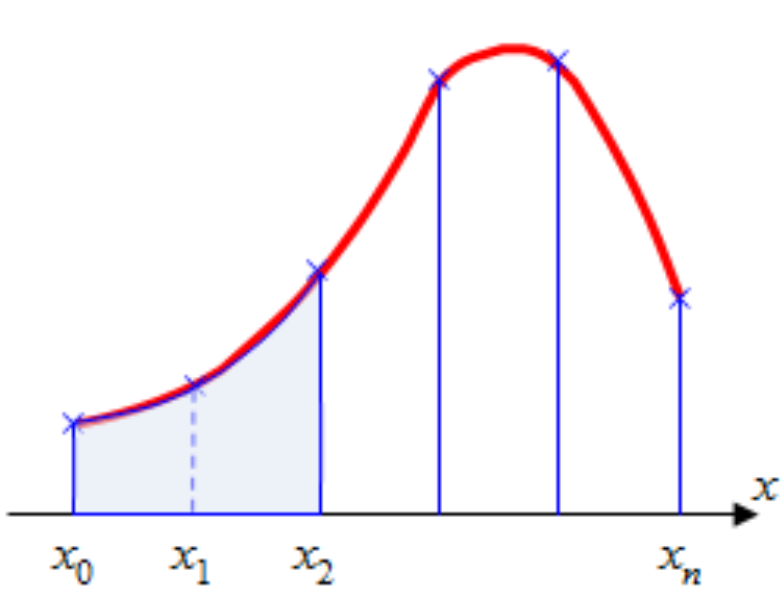
\includegraphics[width=0.65\linewidth]{Pictures/Simpson}
			\caption{Метод Симпсона}
			\label{Simpson}
		\end{figure}
		
		Оказывается, что порядок этого метода скакнул еще выше -- он равен 4. Для сетки с равномерным шагом $h$ и четным количеством интервалов $n$ имеется формула:
		\begin{equation}
			I = \int\limits_{x_0}^{x_n} f(x) dx \approx \frac{h}{3} \left[f_0 + f_n + 4\sum\limits_{k = 1}^{n/2}f_{2k-1} + 2\sum\limits_{k=1}^{n/2 - 1}f_{2k}\right]
		\end{equation}
	
		В общем случае, когда сетка неравномерна и шаги определяются следующим образом: $h_k = x_{k+1} - x_k$, $\overline{0, n-1}$; формула становится немного сложнее:
		\begin{equation}
			 \sum\limits_{k = 0}^{n/2 - 1}\frac{h_{2k} + h_{2k+1}}{6}\left[\left(2 - \frac{h_{2k+1}}{h_{2k}}\right)f_{2k} + \frac{(h_{2k} + h_{2k+1})^2}{h_{2k}h_{2k+1}}f_{2k+1} + \left(2 - \frac{h_{2k}}{h_{2k+1}}\right)f_{2k+2}\right]
		\end{equation}
	
		Если ситуация еще сложнее -- число интервалов $n$ нечетно, то формула выше применяется до предпоследнего интервала, а самый последний считается отдельно добавлением следующих слагаемых:
		\begin{equation*}
			I_\text{full} = I_\text{even} + \alpha f_{n-2} + \beta f_{n-1} + \gamma f_n,
		\end{equation*}
		\noindent где
		\begin{align*}
			\alpha &=  \frac{-h_{n-1}^3}{6h_{n-2} (h_{n-2} + h_{n-1})} \\
			\beta  &=  \frac{h_{n-1}^2 + 3h_{n-1}h_{n-2}}{6h_{n-2}} \\
			\gamma &=  \frac{2h_{n-1}^2 + 3h_{n-1}h_{n-2}}{6(h_{n-2} + h_{n-1})}.
		\end{align*}
	
		Для обычного метода Симпсона с четным $n$ и равномерной сеткой ошибка оценивается следующей формулой:
		\begin{equation}
			|R(f)| \leqslant \max\limits_{[x_0, x_n]}|f^{(4)}(x)| \cdot \frac{x_n - x_0}{180}h^4.
		\end{equation}
	
		\tocsubsection{Метод Рунге-Ромберга-Ричардсона}
		Данная модификация обычных методов интегрирования позволяет получить более высокий порядок точности без значительного увеличения числа арифметических действий.
		
		Пусть для вычисления величины интеграла $I$ есть некоторая формула $I_h$ , позволяющая приближенно получить значение $I$ на равномерной сетке с шагом $h$. Величину остатка можно представить в виде:
		\begin{equation*}
			I - I_h = \psi_h \cdot h^p + o(h^{p}),
		\end{equation*}
		\noindent где $p$ -- порядок точности квадратурной формулы, а $\psi_h \cdot h^p$ -- это главный член погрешности.
		
		Проводя расчет по той же формуле, но на другой сетке с шагом $r \cdot h$, получим другое приближенное значение $I_{rh}$ величины $I$:
		\begin{equation*}
			I - I_{rh} = \psi_{rh} \cdot (r \cdot h)^p + o(h^p).
		\end{equation*}
	
		Вычитая второе из первого и полагая, что при малых значениях $h$ постоянные $\psi_h \approx \psi_{rh} = \psi$, получаем:
		\begin{equation*}
			\psi \cdot h^p = \frac{I_h - I_{rh}}{r^p - 1} + o(h^p).
		\end{equation*}
		
		Тогда, подставляя найденную погрешность в изначальную формулу, получим результат с более высокой точностью:
		\begin{equation}
			I = I_h + \frac{I_h - I_{rh}}{r^p - 1} + o(h^p) = \frac{r^p I_h - I_{rh}}{r^p - 1} + o(h^p).
		\end{equation}
	
		\tocsection{Интегрирование таблично заданной функции}
		\tocsubsection{Постановка задачи}
		В качестве примера для практики был взят номер \textbf{VII.9.5 а)}. В нем описана таблично заданная функция $f(x) = \frac{\sin x}{x}$, доопределенная $f(0) = 1$. Изначально было дано всего 9 точек, то есть разбиение на 8 интервалов. Для рассмотрения нечетного количества интервалов была добавлена еще одна точка.

		\begin{table}[h!]
			\centering
			\begin{tabular}{|c|c|}
				\hline
				$x$  & $f(x)$   \\ \hline
				0.00 & 1.000000 \\ \hline
				0.25 & 0.989616 \\ \hline
				0.50 & 0.958851 \\ \hline
				0.75 & 0.908852 \\ \hline
				1.00 & 0.841471 \\ \hline
				1.25 & 0.759188 \\ \hline
				1.50 & 0.664997 \\ \hline
				1.75 & 0.562278 \\ \hline
				2.00 & 0.454649 \\ \hline \hline
				2.25 & 0.345810 \\ \hline
			\end{tabular}
			\caption{Таблично заданная функция}
		\end{table}
	
		Были реализованы методы трапеций и Симпсона, а также поправочная формула Ричардсона.
		
		
		\tocsubsection{Результаты}
		Используя только 9 точек, то есть разбиение на 8 интервалов, получаем следующие результаты:
		\begin{itemize}
			\item Метод трапеций: $\hspace{57mm} I_t = \textcolor{red}{1.60}31443749999998$
			
			\item Метод трапеций с уточнением Ричардсона: $I_R = \textcolor{red}{1.60541}85833333332$
			
			\item Метод Симпсона: $\hspace{56mm}  I_S = \textcolor{red}{1.60541}85833333332$
		\end{itemize}
		
		Истинное значение: $I_\text{true} = 1.605412976802695...$

		Максимальное отличие от истинного значения составляет $\thicksim 0.14 \%$.	
	
		\newpage
		Теперь используем еще и десятую точку для сравнения методов при нечетном количестве интервалов. Получаем:
		\begin{itemize}
			\item Метод трапеций: $\hspace{57mm} I_t = \textcolor{red}{1.70}32017499999998$
			
			\item Метод трапеций с уточнением Ричардсона: $I_R = \textcolor{red}{1.7054}687812499998$
			
			\item Метод Симпсона: $\hspace{56mm}  I_S = \textcolor{red}{1.705}5011666666666$
		\end{itemize}

		Истинное значение: $I_\text{true} = 1.705457197538423...$
		
		Максимальное отличие от истинного значения составляет $\thicksim 0.14 \%$.	
		
		\newpage
		\tocsection{Вывод}
		В данной работе были проанализированы и реализованы некоторые методы численного интегрирования для функции, заданной табличным образом. А именно -- методы трапеций и Симпсона, а также формула уточнения Ричардсона. Полученные результаты действительно сходятся с заявленным теорией -- порядок формулы Симпсона выше, чем у метода трапеций, а при использовании уточнения Ричардсона точность метода увеличивается. 
		
		Ошибки даже у метода трапеций весьма малы. Они составляют для него в нашем случае $\thicksim 0.14 \%$.
\end{document}